\begin{figure}[h]
\begin{center}
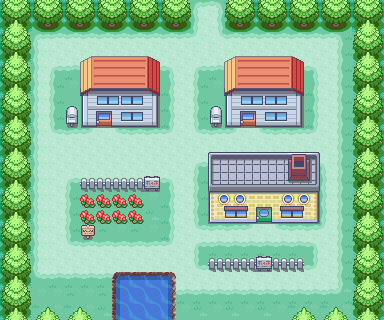
\includegraphics[width=2in]{PokemonPalletTown.png}
\end{center}
\caption{Pallet Town map from Pok\'{e}mon FireRed \cite{firered}} 
\label{fig:pokemon}
\end{figure}

\begin{table}
\label{table:symbols}
\caption{Symbol names and the hand drawn forms}
\begin{center}
\begin{tabular}{llll}
Water & 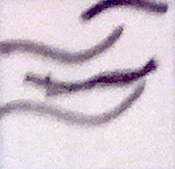
\includegraphics[width=.5in]{water.png} &
Grass & 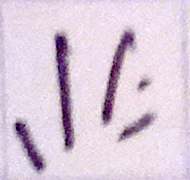
\includegraphics[width=.5in]{grass.png} \\
Rock & 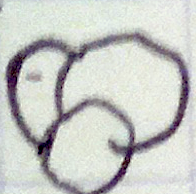
\includegraphics[width=.5in]{rocks.png} &
Tree & 
\includegraphics[width=.5in]{tree.png} \\
Dirt & 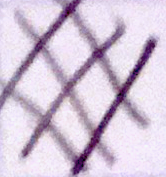
\includegraphics[width=.5in]{dirt.png} &
Sand & 
\includegraphics[width=.5in]{sand.png} \\
\end{tabular}
\end{center}
\end{table}

We have created 6 symbols to be used in recreating maps from the popular video
game Pok\'{e}mon. Choosing a specific source ensures that our data set is
sampled from a well defined distribution.  An example map from the game is
shown in Figure \ref{fig:pokemon}. There is a sample of the symbol names and
the hand drawn forms in Table \ref{table:symbols}.


